
\section{Overview of the CBM experiment}

\gls{CBM} is well positioned to explore many facets of \gls{QCD} matter, and to discover new exotic states (in combination with \gls{PANDA} experiment). In addition, it will be able to explore the equation of sta  te at densities and temperatures close to those probed by neutron star mergers. The \gls{CBM} aims to study the following physics phenomenon:
\begin{itemize}
    \item the equation of state of baryonic matter at neutron star densities,
    \item in-medium properties of hadrons which are modified by the restoration of chiral symmetry in the dense baryonic matter, 
    \item phase transitions from hydronic matter to quarkonic or partonic matter,
    \item hypernuclei,
    \item charm production mechanisms.
\end{itemize}



\begin{figure}[!h]
    \centering
    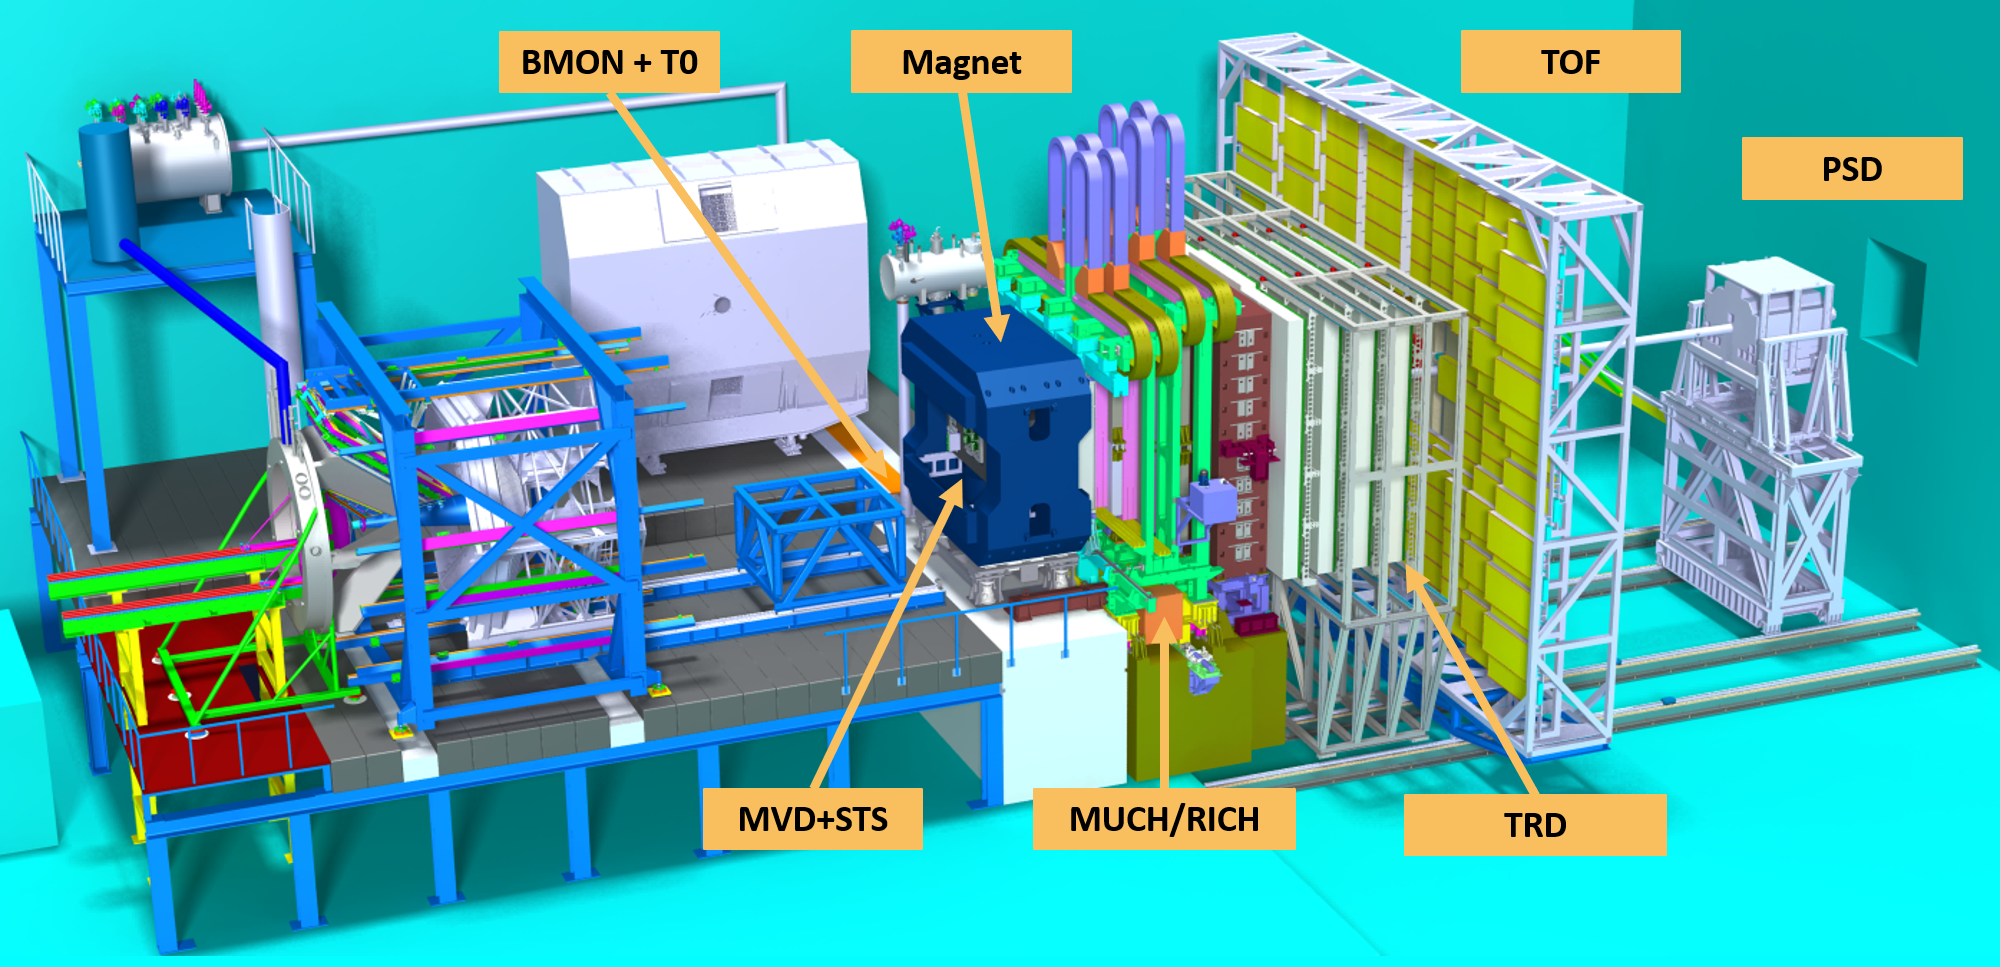
\includegraphics[width=0.95\columnwidth]{Chapter1/images/CBMnew.png}
    \caption{HADES experiment on the left side and the \gls{CBM} experiment on the right side}.
    \label{fig:exp}
\end{figure}

Construction of the Compressed Baryonic Matter (\gls{CBM}) experiment is currently underway at \gls{FAIR}. Figure~\ref{fig:exp} depicts the CAD drawing of the \gls{CBM} experiment. The beam enters the experimental cave from the left side and traverses the High Acceptance Di-Electron Spectrometer (\gls{HADES}) experiment.  The main features of the \gls{CBM} experiment are described below:
\begin{itemize}
\item tracking acceptance: $\SI{2.5}{\degree} < \theta_{lab} < \SI{25}{\degree}$,
\item peak intensities reach 10 MHz for Au+Au systems,
\item fast and radiation hard detectors,
\item free-streaming \gls{DAQ},
\item 4D tracking,
\item online event reconstruction and selection,
\item data rates up to 1~TB/s.
\end{itemize}




The CBM detector system can be used in two operation modes: the first one is optimized for electron identification (electron configuration) and the second is specialized for muon identification (muon configuration). In the first one, all the subsystems apart from MUCH will be involved. In the muon configuration, the \gls{RICH} detector is replaced by \gls{MUCH}.



The experiment consists of the following detectors:

\textbf{Beam monitor, or T0 (\gls{BMON})} and its conceptual design, was summarized during the 40th \gls{CBM} Collaboration Meeting~\cite{bmon}. Two separate stations in front of the target are made out of high-purity poly-crystalline CVD diamond material. This detector is foreseen to monitor beam quality (position, time structure) and determine the start time of the reaction.

\textbf{Micro Vertex Detector} (\gls{MVD}) consists of four planar stations with Monolithic Active Pixel Sensor (\gls{MAPS}) chips. A station's layout and distance from the target can be tailored to the needs of a specific run, for example, to optimize vertexing or tracking. The vertexing detector geometry aims at a precision of secondary vertices determination of about 50 -- 100~$\mu m$ along the beam axis. The main aims cover decay vertex identification of the very short-lived particles such as charmed mesons, which decay within a few hundred $\mu m$ behind the target, as well as background rejection in di-electron spectroscopy. More information can be found in the Technical Design Review~\cite{MVD}.

 \textbf{Silicon Tracking System} \gls{STS} which is responsible for tracking of charged particles and measuring their momentum. The \gls{STS} is located inside a superconducting dipole magnet~\cite{Malakhov:109025},
 
\textbf{Muon Chamber System} \gls{MUCH} is the fourth subsystem of the \gls{CBM} experiment. It is dedicated to muon detection and track reconstruction.

\textbf{Ring Imaging Cherenkov Detector} \gls{RICH}

\textbf{Transition Radiation Detector} \gls{TRD}

\textbf{Time-of-Flight Detector} \gls{TOF}


\textbf{Projectile Spectator Detector} \gls{PSD}



To read:

For muon measurements, the RICH will be replaced by a Muon Chamber (MuCh) system. The MuCh consists of one hadron absorber made of graphite, followed by up to four iron plates, with muon tracking detector triplets behind each absorber. The circular detector triplets behind the first two absorbers, where the particle rate still is up to 500 kHz/cm2, are composed of 18 and 20 trapezoidal Gas Electron
Multiplier (GEM) detectors per layer. The third and fourth triplet, where the particle rate is decreased to about 15 and 4 kHz/cm2, will be built from single-gap RPC detectors with low-resistivity Bakelite electrodes.

Behind the fifth iron absorber, the muons will be tracked by the TRD and finally identified by the TOF. The event characterization, that is, the determination of the reaction plane angle and the centrality, will be performed by the Project Spectator Detector (PSD), a segmented hadron calorimeter located about 10 m downstream of the target.

For the high-rate CBM experiment, the data read-out and acquisition system plays a crucial role. As mentioned above, the time-stamped signals will be read out without event correlation and transferred to a high-performance computing farm, the GSI GreenIT Cube, where online event reconstruction and selection are performed by high-speed algorithms. In the first step, the tracks of the charged particles were reconstructed from the space and time information of the various detector signals. In a second step, the particles will be identified, taking into account secondary decay vertices and information of RICH or MuCh, TRD, and TOF. Finally, the particles will be grouped into events, which will be selected for storage if they contain important observable. In parallel, the event is characterized using information from the PSD.



\section{Thesis overview and its rationale}
The thesis is divided into 7 chapters. The second chapter introduces the role of silicon trackers in large scientific experiments and brings the design details of the \gls{STS} closer, including the physics performance and experimental challenges. Those elements are directly connected with the requirements for the Detector Control System (\gls{DCS}). The third chapter serves as an introduction to how to control and monitor a large experiment, with an extended focus on the detector-related slow control system and the developed control framework. The next three chapters are focused on the results and their consequences for the experiment:
\begin{itemize}
    \item chapter 4 covers the first implementations of the mentioned control framework. The first application is related to the slow control interface for the \gls{FEE} readout. The second and third examples are related to the irradiation studies of the powering modules for the \gls{LV} powering of the \gls{STS} electronics and thermal cycling of \glspl{FEB}. The performed studies and results of these activities are discussed in detail,
    \item chapter 5 describes the efforts to design and test a distributed sensing system for the \gls{STS} with a focus on humidity sensing. Three considered technologies feature capacitive sensors, fiber optic sensors, and remote sensing with the use of a sampling system. The chapter focuses on the design choices and characterization of the fiber Bragg grating-based sensors. 
    \item chapter 6 focuses on the small-scale prototype version of the \gls{STS} in the \gls{mCBM} experiment. The first sections describe in detail the hardware and software solutions implemented in the detector. Subsequently, the results from the full-blown \gls{DCS} are presented and discussed, including the radiation effects on the silicon sensors and general considerations about the power dissipation of different elements of the \gls{STS}'s powering scheme. Moreover, considerations about the \gls{DCS} are given. 
\end{itemize}
The last part of the thesis summarizes the results and sheds a light on the next steps toward the realization of the \gls{STS} and its controls. The most important findings and results from the performed studies are also discussed.